% !TeX spellcheck = de_DE
\clearpage
\section{\ExercisePrefixEmbeddedC Joysticks abfragen \optional}

\optionaltextboxC

In diesem Abschnitt nutzen wir die Funktionen der vorigen Aufgabe, um die analogen Werte der Joysticks auszugeben. Darauf aufbauend entwickelst du eine Aufgabe, die mithilfe des Joysticks die Farbe der RGB-LED verändert.
Die zu implementierenden Funktionen befinden sich in der Datei \filename{joystick.c}.
Solltest du die vorherige Aufgabe nicht (vollständig) bearbeitet haben, kannst du auf die Musterlösung in der Datei \filename{display\_s.c} zurückgreifen.
Um diese statt deiner eigenen Lösung zu nutzen, hängst du an jeden Funktionsnamen das Suffix \filename{\_s} an (\bspw \lstinline|writeChar_s| statt \lstinline|writeChar|).

\subsection{Analoge Werte auf dem Display anzeigen}

Jeder Joystick besitzt zwei analoge Leitungen, welche die X- oder Y-Position des Steuerknüppels auslesen.
Die analogen Werte entsprechen dabei der Spannung des jeweiligen Drehpotentiometers der Achse, welche zwischen \SI{0}{\volt} und \SI{5}{\volt} liegt.
Die Spannungswerte der Joysticks werden durch den Analog-Digital-Wandler des Microcontrollers auf einen 8-Bit-Wert abgebildet (Wertebereich: 0 bis 255).
Die Aufteilung der Wertebereiche sowie die Orientierung der X- und Y-Richtung sind in Abbildung \ref{fig:jostickValues} dargestellt.
%
\begin{figure}[!htb]
    \begin{centering}
        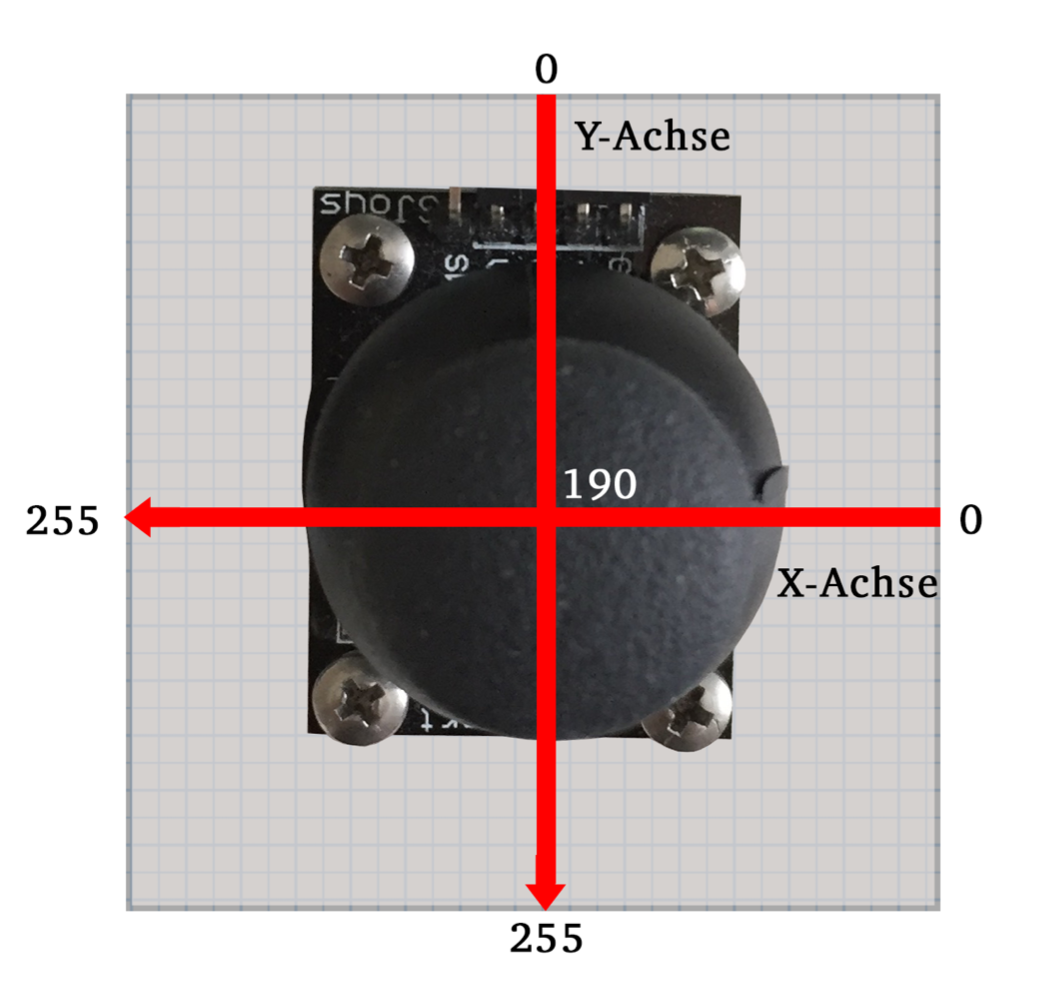
\includegraphics[width=.4\textwidth]{./05_c/figures/joystickValues.png}
        \caption{Wertebereich der Joysticks}
        \label{fig:jostickValues}
    \end{centering}
\end{figure}
%
Die Aufteilung ist nicht gleichmäßig.
Stattdessen ergibt sich in Neutralstellung der Wert $(190,190)$.
Joystick 1 ist mit den analogen Anschlüssen AN16 (X) und AN19 (Y) und Joystick 2 ist mit AN13 (X) und AN23 (Y) verbunden. 

\begin{enumerate}
\item
Implementiere die Funktion \lstinline|printValues|, welche über Zeiger auf die analogen Leitungen AN13, AN16, AN19 und AN23 die Werte der Joysticks ausliest und diese auf dem Bildschirm ausgibt.  
Nutze dazu die Funktionen in Tabelle \ref{tab:joystickInfo} und folgendes Codefragment, mithilfe dessen man die Analog-Kanäle ausliest:

\cpppInputListing{05_c/listings/readAnalog.c}

\item 
Um fortlaufend die Positionsdaten des Joysticks auszugeben, rufe \lstinline|printValues| in einer Schleife auf:

\cpppInputNoPageBreakListing{05_c/listings/joystick_example.c}
\end{enumerate}

\begin{table}[!htb]
    \centering
    \caption{Wichtige Funktionen und Variablen für die Verwendung der Joysticks}
    \label{tab:joystickInfo}
    \begin{tabular}{p{7cm}p{7cm}}
        \toprule
        \textbf{Funktionen/Variablen} & \textbf{Beschreibung} \\
        \midrule
        \lstinline|setCursor(0, 319)| & Setzt den Cursor auf die linke obere Ecke\\
        \lstinline|void writeTextln(char *text)| & Schreibt \lstinline|text| auf das Display und verschiebt den Cursor mit Zeilensprung \\
        \lstinline|void writeText(char *text)| & Schreibt \lstinline|text| auf das Display und verschiebt den Cursor ohne Zeilensprung \\
        \lstinline|void writeNumberOnDisplayRight(const uint8_t *number)| & Schreibt die per Pointer referenzierte Zahl \lstinline|number| an die Position des Cursors und verschiebt den Cursor\\
        \bottomrule
    \end{tabular}
\end{table}


\subsection{LED mit Joystick 1 kontrollieren}
In dieser Aufgabe soll die Funktion \lstinline|controlLEDs| geschrieben werden, um die Farbe der RGB-LED durch die Bewegung des Joysticks 1 nach links oder rechts zu verändern.
\Cref{tab:controlLED} zeigt die verschiedenen möglichen Wertebereiche mit den anzusteuernden Ports und Pins der LEDs (wie in \filename{pins.h} definiert).

\begin{table}[!htb]
    \centering
    \caption{Anzeigebereiche der LEDs}
    \label{tab:controlLED}
    \begin{tabular}{llllr}
        \toprule
        \textbf{Position des Joystick} & 
        \textbf{LED-Farbe} & 
        \textbf{Werebereich AN16} & 
        \textbf{Daten-Port} & 
        \textbf{Ausgabe-Pin}\\
        \midrule
        Links & Grün & 255 \dots 200 & \lstinline|LED_GREEN_DOR| & \lstinline|LED_GREEN_PIN| \\
        Mitte & Blau & 200 \dots 180 & \lstinline|LED_BLUE_DOR| & \lstinline|LED_BLUE_PIN| \\
        Rechts & Rot & 180 \dots 0 & \lstinline|LED_RED_DOR| & \lstinline|LED_RED_PIN| \\
        \bottomrule
    \end{tabular}
\end{table}

\begin{enumerate}
\item
Implementiere zunächst die Hilfsfunktion \lstinline|controlLEDsInit|, welche die Leitungen der RGB-LEDs initialisiert. Die analogen Kanäle der LEDs sollen ausgeschaltet werden.
Definiere die Pins der LEDs als Ausgänge und initialisiere sie mit \lstinline|1u| (= \enquote{aus}). 

\item
Implementiere nun die Funktion \lstinline|controlLEDs|, welche die Position der X-Achse des Joystick über den analogen Kanal AN16 ausliest und die Farbe der RGB-LED gemäß Tabelle \ref{tab:controlLED} verändert. 

\item 
Dein Testcode sollte in etwa wie folgt aussehen:

\cpppInputNoPageBreakListing{05_c/listings/controlLEDs_testcode.c}
\end{enumerate}
